% Superexchange J = 4t^2/U: Pauli-blocked triplet vs virtual double occupancy (Session 1).
% Own drawing (Fable). Compile with: pdflatex superexchange.tex ; result moves to ../superexchange.pdf
\documentclass[11pt,tikz,border=3pt]{standalone}
\usepackage{amsmath,amssymb}
\usepackage{xcolor}
\definecolor{coursedark}{HTML}{1B2A4A}
\definecolor{courseaccent}{HTML}{7A2E8C}

\begin{document}
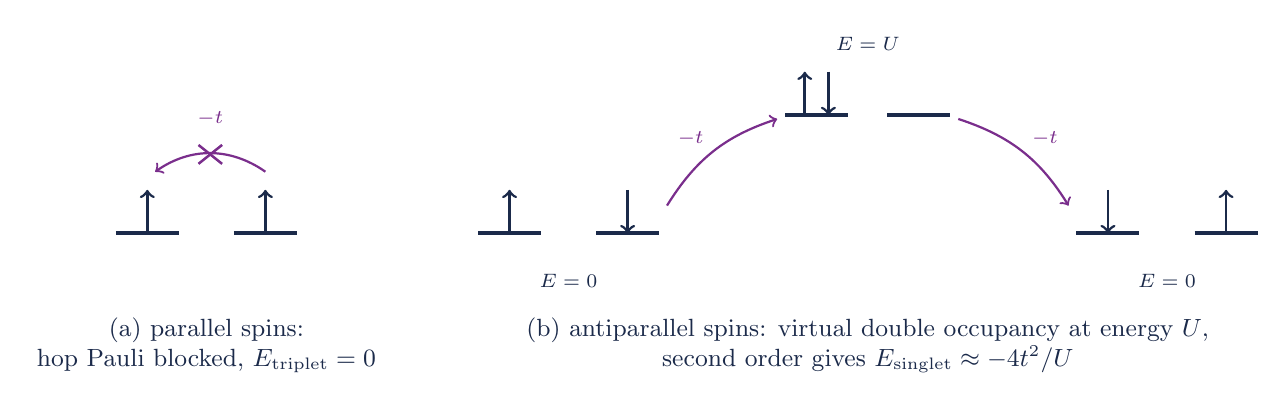
\begin{tikzpicture}[
    level/.style={draw=coursedark, line width=1.3pt},
    spin/.style={->, draw=coursedark, line width=1.0pt},
    hop/.style={->, draw=courseaccent, line width=0.8pt},
    lbl/.style={font=\small, text=coursedark, align=center},
    idx/.style={font=\scriptsize, text=coursedark, align=center},
  ]

  % ---- panel (a): parallel spins, Pauli blocked
  \begin{scope}[shift={(0,0)}]
    \draw[level] (0,0) -- (0.8,0);   \draw[level] (1.5,0) -- (2.3,0);
    \draw[spin] (0.4,0) -- (0.4,0.55);
    \draw[spin] (1.9,0) -- (1.9,0.55);
    \draw[hop] (1.9,0.78) to[bend right=35] (0.5,0.78);
    \draw[courseaccent, line width=0.9pt] (1.05,0.88) -- (1.35,1.12);
    \draw[courseaccent, line width=0.9pt] (1.05,1.12) -- (1.35,0.88);
    \node[idx, text=courseaccent] at (1.2,1.45) {$-t$};
    \node[lbl, anchor=north] at (1.15,-0.95)
      {(a) parallel spins:\\ hop Pauli blocked, $E_{\mathrm{triplet}}=0$};
  \end{scope}

  % ---- panel (b): antiparallel spins, virtual double occupancy at energy U
  \begin{scope}[shift={(4.6,0)}]
    % initial state
    \draw[level] (0,0) -- (0.8,0);   \draw[level] (1.5,0) -- (2.3,0);
    \draw[spin] (0.4,0) -- (0.4,0.55);
    \draw[spin] (1.9,0.55) -- (1.9,0);
    \node[idx, anchor=north] at (1.15,-0.40) {$E=0$};
    % virtual state, elevated
    \draw[level] (3.9,1.5) -- (4.7,1.5);   \draw[level] (5.2,1.5) -- (6.0,1.5);
    \draw[spin] (4.15,1.5) -- (4.15,2.05);
    \draw[spin] (4.45,2.05) -- (4.45,1.5);
    \node[idx, anchor=south] at (4.95,2.2) {$E=U$};
    % final state
    \draw[level] (7.6,0) -- (8.4,0);   \draw[level] (9.1,0) -- (9.9,0);
    \draw[spin] (8.0,0.55) -- (8.0,0);
    \draw[spin] (9.5,0) -- (9.5,0.55);
    \node[idx, anchor=north] at (8.75,-0.40) {$E=0$};
    % hops
    \draw[hop] (2.4,0.35) to[bend left=20] (3.8,1.45);
    \node[idx, text=courseaccent] at (2.70,1.20) {$-t$};
    \draw[hop] (6.1,1.45) to[bend left=20] (7.5,0.35);
    \node[idx, text=courseaccent] at (7.20,1.20) {$-t$};
    \node[lbl, anchor=north] at (4.95,-0.95)
      {(b) antiparallel spins: virtual double occupancy at energy $U$,\\
       second order gives $E_{\mathrm{singlet}}\approx-4t^2/U$};
  \end{scope}
\end{tikzpicture}
\end{document}
